\chapter{Calculations for Harmonic Motion Problems}
\label{appendix:harmonic-motion}

In this appendix, we will show some of the calculus that we used to generate
the graphs in Chapter~\ref{chapter:harmonic-motion}.


\begin{figure}[ht]
  \centering
  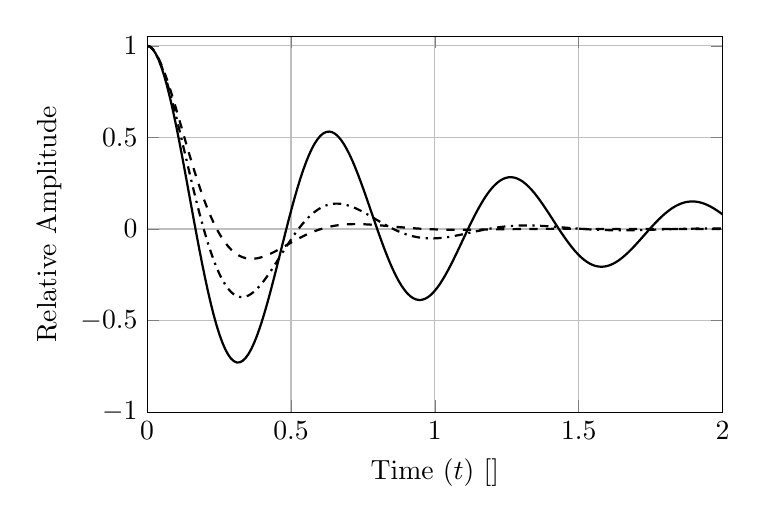
\begin{tikzpicture}
    \begin{axis}[
        width=3.5in,
        height=2.5in,
        xmin=0,xmax=2,
        xlabel={Time ($t$) [\si\second]},
        ymin=-1,
        ymax=1.05,
        ylabel={Relative Amplitude},
        grid=both,
      ]
      \addplot[
        samples=200,
        domain=0:2,
        thick]{1.005*exp(-x)*cos(deg(sqrt(99)*x)-5.74)};
      \addplot[
        samples=200,
        domain=0:2,
        thick,dash dot]{1.048*exp(-3*x)*cos(deg(sqrt(91)*x)-17.46)};
      \addplot[
        samples=200,
        domain=0:2,
        thick,dashed]{1.154*exp(-5*x)*cos(deg(sqrt(75)*x)-30)};
      %\addplot[
      %  color=red,
      %  samples=100,
      %  domain=0:1.6,
      %  thick]{(1+10*x)*exp(-10*x)};
      %%\addlegendentry{Critically damped ($b=b_c$)}
      %\addplot[
      %  color=pink,
      %  samples=100,
      %  domain=0:1.6,
      %  thick]{1.077*exp(-2.679*x)-0.077*exp(-37.32*x};
      %%\addlegendentry{Over damped ($b=2b_c$)}
    \end{axis}
  \end{tikzpicture}
  \caption{Effects of damping factor $b$ on an under-damped oscillator}
  \label{fig:damping-effects-appendix}
\end{figure}

\subsubsection*{Under-Damped Oscillator}
For the under-damped oscillator with $b<\sqrt{4mk}$, the solution $x(t)$ has
both an exponential decay term and a sinusoidal (oscillatory) term:
\begin{equation}
  x(t)= a e^{-\lambda t}\cos(\omega' t+\theta_0)
  \label{eq:appendix-damped-position}
\end{equation}
where, from Eq.~\ref{damping1}:
\begin{equation*}
  \lambda=\frac b{2m}\quad\text{and}\quad
  \omega'=\sqrt{\omega^2-\lambda^2}
\end{equation*}
In Fig.~\ref{fig:damping-effects} (reproduced for the under-damped oscillator in
Fig.~\ref{fig:damping-effects-appendix}), we plotted the solutions $x(t)$ with
various damping factors $b$. In every case, motion starts at amplitude
(i.e.\ $x(0)=A_0$) from rest (i.e.\ $v(0)=\dot x(0)=0$). For simple harmonic
oscillators ($b=0$), we can just use  a cosine function, and setting $a=A_0$
and $\theta_0=0$. However, for the damped oscillator, as the exponential term
in Eq.~\ref{eq:appendix-damped-position} does not have a zero slope at $t=0$,
the phase constant must be nonzero. Instead, we have to apply both initial
position and velocity to find $a$ and $\theta_0$. Starting with the initial
position, we can substitute $t=0$ into Eq.~\ref{eq:appendix-damped-position}
to get $a$:
\begin{equation}
  x(0)= a \cancel{e^{-\lambda t}}\cos(\cancel{\omega't}+\theta_0)=A_0
  \quad\quad\longrightarrow\quad\quad
  a=\frac{A_0}{\cos\theta_0}
\end{equation}
Which still requires us to find the phase constant $\theta_0$. Taking the time
derivative (and don't forget to apply the product rule and chain rule
properly!) of Eq.~\ref{eq:appendix-damped-position} gives us the velocity
$v(t)$ of the motion, which is considerably a more complicated expression than
the simple harmonic oscillator:
\begin{equation}
  v(t)=\diff xt
  = -ae^{-\lambda t}\left[
    \lambda\cos(\omega' t+\theta_0)
    +\omega'\sin(\omega' t+\theta_0)
    \right]
  \label{eq:appendix-damped-velocity}
\end{equation}
Setting the initial condition $v(0)=0$ at $t=0$, and after bit of algebra and
trigonometry that will be left to you, we find the phase constant $\theta_0$:
\begin{equation}
  v(0) =-a\cancel{e^{-\lambda t}}
  \left[
    \lambda\cos(\cancel{\omega't}+\theta_0)+
    \omega'\sin(\cancel{\omega't}+\theta_0)
    \right]=0
  \quad\longrightarrow\quad
  %0 &=\lambda\cos(\theta_0)+\omega'\sin(\theta_0) \\
  %-\lambda\cos(\theta_0) &= \omega\sin(\theta_0) \\
  %-\frac{\lambda}{\omega'} &=\tan(\theta_0)\\
  \theta_0 =\tan^{-1}\left[-\frac\lambda{\omega'}\right]
\end{equation}
%To satisfy the initial conditions, the phase constant is not zero.
Our final equation for the position for the under-damped oscillator, which is
plotted in Fig.~\ref{fig:damping-effects}, is now:
\begin{equation}
  x(t)=\left[\frac{A_0}{\cos\theta_0}\right] e^{-\lambda t}\cos(\omega't+\theta_0)
  \label{eq:underdamped-final}
\end{equation}
Both Fig.~\ref{fig:damping-effects} and Fig.~\ref{fig:damping-effects-appendix}
were plotted for an example case with a spring constant of
$k=\SI{100}{\newton\per\metre}$, a mass of $m=\SI1{\kilo\gram}$ and initial
amplitude $A_0=1$. The undamped natural frequency is
$\omega=\sqrt{k/m}=\SI{10}{rad\per\second}$. In
Table~\ref{tabl:damping-parameters}, we use these values to calculate $\lambda$,
$\omega'$ and $\theta_0$ which are then substtituted back into
Eq.~\ref{eq:underdamped-final} and plotted in
Fig.~\ref{fig:damping-effects-appendix}.
\begin{table}[ht]
  \centering
  \begin{tabular}{ccc}
    {\sffamily$b$} &
    {\sffamily$\lambda=\dfrac b{2m}$} &
    {\sffamily$\omega'=\sqrt{\omega^2-\lambda^2}$} \\
    \hline\hline
    $0.1b_c$ & 1 & $\sqrt{99}$ \\
    $0.3b_c$ & 3 & $\sqrt{91}$ \\
    $0.5b_c$ & 5 & $\sqrt{75}$ \\
    $b_c$ & 10 & N/A \\
    \hline
  \end{tabular}
  \caption{Damping parameter and pseudo frequency for the under-damped
    oscillator}
  \label{tabl:damping-parameters}
\end{table}
%where $A_0$ is the initial amplitude. Like the simple harmonic oscillator,
%$A_0$, $\theta_0$, and whether to use a sine or cosine function, are based on
%initial conditions. The motion of the mass is called a
%\textbf{damped harmonic motion}, and such a system is called a
%\textbf{damped harmonic oscillator}.
%
%Unlike the simple harmonic oscillator, the motion of the damped oscillator is
%\emph{quasi}-periodic because the oscillation pattern is not perfectly
%repeated. The natural frequency\footnote{Because the motion is quasi-periodic,
%this frequency should be properly called a ``quasi-frequency''.} $\omega'$ for
%the damped oscillator is shifted from the undamped case $\omega$ based on the
%damping factor $b$:
%\begin{important-equation}
%  \quad\text{where}\quad
%  \omega=\sqrt{\frac km}
%  \label
%\end{important-equation}
%Note that $\omega'<\omega$ (natural frequency decreases) because of the
%damping factor $b$.



\subsubsection*{Critically Damped}
At critical damping, where $b=b_c=\sqrt{4mk}$, our solution is in the form:
\begin{equation}
  x(t)=(c_1+c_2t)e^{-\lambda t}
\end{equation}
Again, with $\lambda$ defined the same way. Again, we want to find the solution
$x(t)$ with motion starting at amplitude ($x(0)=A_0$) from rest (i.e.\
$v(0)=\dot x(0)=0$). Substituting $x(0)=0$ into the above euqation, we can
easily find that 
\begin{equation}
  x(0)=(c_1+\cancel{c_2t})\cancel{e^{-\lambda t}}=A_0
  \quad\to\quad
  c_1=A_0
\end{equation}
Again, we take the derivative of $x$ with respect to time, and using product
rule and chain rule, we find the velocity profile ($v(t)$) to be:
\begin{equation}
  v(t)=\diff xt=-(c_2\lambda t +c_1\lambda -c_2)e^{-\lambda t}
\end{equation}
putting in initial conditions
\begin{equation}
  v(0)=-(\cancel{c_2\lambda t} +c_1\lambda -c_2)\cancel{e^{-\lambda t}}=0
\end{equation}
which leads us to the equation:
\begin{equation}
  c_1\lambda -c_2=0\quad\to\quad c_2=c_1\lambda=A_0\lambda
\end{equation}
The final solution is
\begin{equation}
  x(t)=A_0(1+\lambda t)e^{-\lambda t}
\end{equation}

%\begin{important-equation}
%\end{important-equation}
%At critical damping, the solution to Eq.~\ref{eq:ode2} for the position of the
%mass $x(t)$ is
%where $c_1$ and $c_2$ are determined by initial conditions. If a mass is
%released at amplitude $A_0$ from rest (i.e.\ $x(0)=A_0$, $\dot x(0)=0$), then
%Eq.~\ref{eq:critically-damped-solution} becomes:
%\begin{equation}
%  x(t)=\left[A_0+\frac{\lambda}A_0\right]e^{-\lambda t}
%  \label{eq:critically-damped-solution-2}
%\end{equation}
%\begin{remark}
%  The solution in Eq.~\ref{eq:critically-damped-solution} are really two
%  linearly independent solutions:
%  \begin{align*}
%    x_1(t) &= c_1e^{\frac{b_ct}{2m}} \\
%    x_2(t) &= c_2te^{\frac{b_ct}{2m}}
%  \end{align*}
%  We should not be surprised that both solutions are also orthogonal functions.
%\end{remark}
%A critically damped system returns to its equilibrium position in the shortest
%time with \emph{no} oscillation.
%\textbf{EXPAND ON THIS SECTION: Critical or near-critical damping is desired
%in many engineering designs (e.g.\ shock absorbers on car suspensions).}

\subsubsection*{Over-Damped}

For the over-damped system, where $b>\sqrt{4mk}$, the solution $x(t)$ is the
linear combination of \emph{two} exponential decay functions.
\begin{equation}
  x(t)=c_1e^{r_1t}+c_2e^{r_2t}
\end{equation}
where
\begin{equation*}
  r_1=\frac{-b+\sqrt{b^2-4mk}}{2m}\quad
  r_2=\frac{-b-\sqrt{b^2-4mk}}{2m}
\end{equation*}
We can easily verify that both roots $r_1$ and $r_2$ are real and negative.
With initial condition $x(0)=A_0$, we have
\begin{equation}
  x(0)=c_1\cancel{e^{r_1t}}+c_2\cancel{e^{r_2t}}=0
  \quad\quad\longrightarrow\quad\quad
  c_1+c_2=A_0
\end{equation}
Taking the derivative with respect to time, we have
\begin{equation}
  v(t)=\diff xt=r_1c_1e^{r_1t}+r_2c_2e^{r_2t}
\end{equation}
With initial condition $v(0)=0$, we have a second equation:
\begin{equation}
  v(0)=r_1c_1+r_2c_2=0
\end{equation}
To find the full solution, we solve the set of linear equations:
\begin{align*}
  c_1 + c_2 &= A_0\\
  c_1r_1 + c_2r_2 &=0
\end{align*}
